\begin{frame}
	\frametitle{Kalman Filter}
	\note{información extraida de https://youtu.be/PiCC-SxWlH8}
	
	\begin{itemize}
		\item Es un Filtro de Bayes
		\item Todo es Gaussiano
		\begin{equation*}
			p(x)=\det(2\pi\covariance)^{\frac{1}{2}} \exp\left(-\dfrac{1}{2} (x - \mu )^{\top} \inverse{\covariance} (x - \mu )  \right)
		\end{equation*}
		
		\item Soluciones optimas para modelos lineales y distribuciones Gaussianas.
	\end{itemize}

	\begin{figure}[!h]
		\centering
		\subfloat[]
		{
			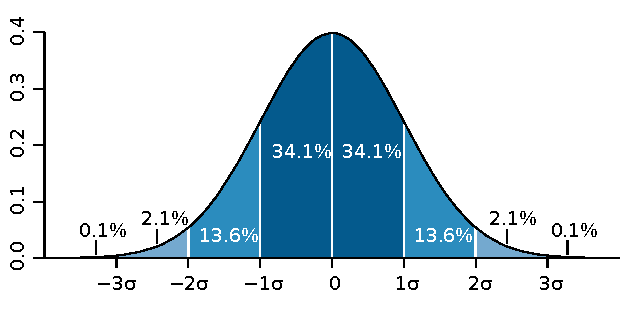
\includegraphics[width=0.3\columnwidth]{./images/standard_deviation_diagram.pdf}
		}
		\subfloat[]
		{
			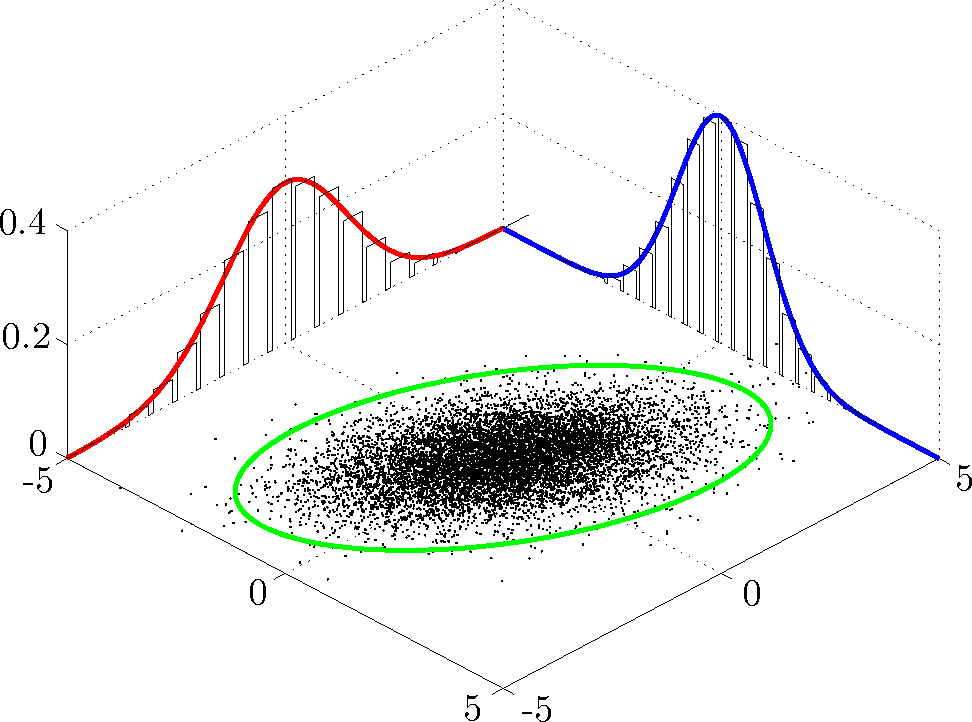
\includegraphics[width=0.3\columnwidth]{./images/multivariate_normal_sample.pdf}
		}
		\subfloat[]
		{
			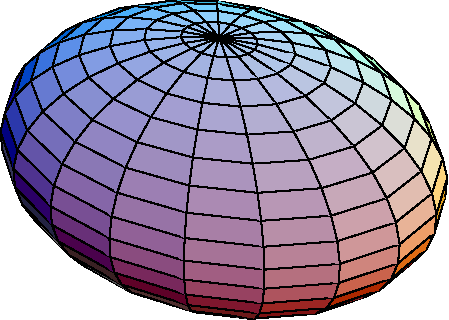
\includegraphics[width=0.2\columnwidth]{./images/ellipsoid.pdf}
		}
	\end{figure}
\end{frame}


\begin{frame}
	\frametitle{Suposiciones de Kalman Filter}
	\note{información extraida de https://youtu.be/PiCC-SxWlH8}
	
	\begin{itemize}
		\item Ruido y distribuciones Gaussianas
		\item Modelos de movimiento y observación lineales
	\end{itemize}

	\begin{align*}
		\state_{t} &= A_{t} \state_{t-1} + B_{t}\controlCommand_{t} + \motionModelNoise_{t}\\
		\observation_{t} &= C_{t} \state_{t} + \measurementModelNoise_{t}
	\end{align*}
	\note{Kalman Filter requiere que los ruidos sean gaussianos y que el estado resulte de una combinación lineal.}

	\centering
	\alert{¿qué pasa si este estas suposiciones no pasan?}
	\note{Differencial drive y Ackerman motion models NO son modelos lineales}
	\note{Los observation models de un láser  o de una cámara tampoco son lineales.}
\end{frame}

\begin{frame}
	\frametitle{Sistemas dinámicos no Non-lineales}
	\note{información extraida de https://youtu.be/PiCC-SxWlH8}
	\begin{itemize}
		\item Los problemas reales en general emplean funciones no-lineales
	\end{itemize}
	
%	\begin{align*}
%		\state_{t} &= A_{t} \state_{t-1} + B_{t}\controlCommand_{t} + \motionModelNoise_{t}\\
%		\observation_{t} &= C_{t} \state_{t} + \measurementModelNoise_{t}
%	\end{align*}

	\begin{figure}[!h]

		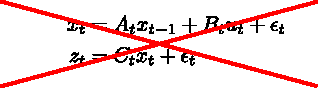
\includegraphics[width=0.4\columnwidth]{./images/kalman_filter_linear_equations_cross_out.pdf}
	\end{figure}

	\begin{align*}
		\state_{t} &= \motionModelFunction{\controlCommand_{t}, \state_{t-1}} + \motionModelNoise_{t}\\
		\observation_{t} &= \observationModelFunction{\state_{t}} + \measurementModelNoise_{t}
	\end{align*}

\end{frame}


\begin{frame}
	\frametitle{Filtro de Kalman 1D}
	\note{información extraida de https://youtu.be/E-6paM_Iwfc}
	
	\begin{figure}[!h]
		\centering
		\subfloat[Predicción Inicial]
		{
			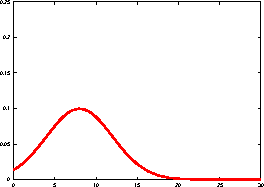
\includegraphics[width=0.3\columnwidth]{./images/kalman_filter_initial_prediction.pdf}
		}
		\subfloat[Medición]
		{
			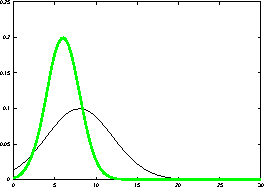
\includegraphics[width=0.3\columnwidth]{./images/kalman_filter_first_measurement.pdf}
		}
		\subfloat[Corrección]
		{
			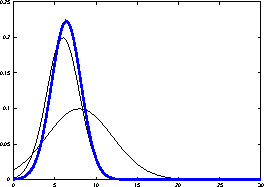
\includegraphics[width=0.3\columnwidth]{./images/kalman_filter_first_correction.pdf}
		}
	\end{figure}
	
\end{frame}

\begin{frame}
	\frametitle{Filtro de Kalman 1D}
	\note{información extraida de https://youtu.be/E-6paM_Iwfc}
	
	\begin{figure}[!h]
		\centering
		\subfloat[Predicción por Movimiento]
		{
			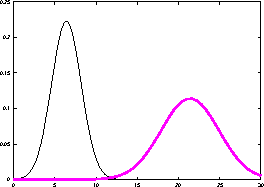
\includegraphics[width=0.3\columnwidth]{./images/kalman_filter_motion_prediction.pdf}
		}
		\subfloat[Segunda Medición]
		{
			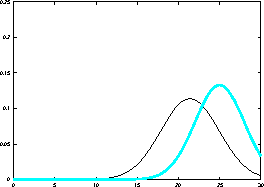
\includegraphics[width=0.3\columnwidth]{./images/kalman_filter_second_measurement.pdf}
		}
		\subfloat[Segunda Corrección]
		{
			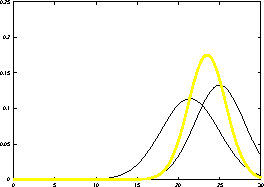
\includegraphics[width=0.3\columnwidth]{./images/kalman_filter_second_correction.pdf}
		}
	\end{figure}
	
\end{frame}


\begin{frame}
	\frametitle{Linearización en EKF: Expansión de Taylor de primer orden}
	
	\TODO{Agregar slides \url{https://www.youtube.com/watch?v=E-6paM\_Iwfc\&t=3260s}}
\end{frame}


\begin{frame}
	\frametitle{Suposición de Linealidad}
	
	\begin{figure}[!h]
		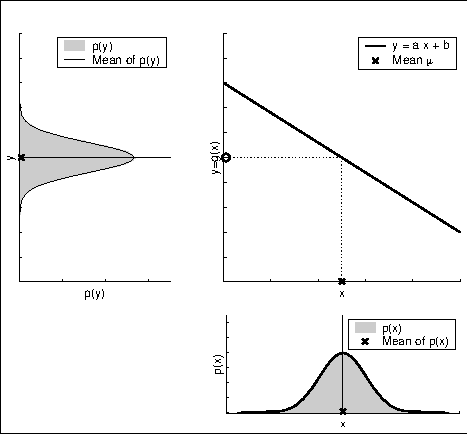
\includegraphics[width=0.5\columnwidth]{./images/linear_transformation_of_a_gaussian.pdf}
	\end{figure}
\end{frame}

\begin{frame}
	\frametitle{Función No-Lineal}
	
	\begin{figure}[!h]
		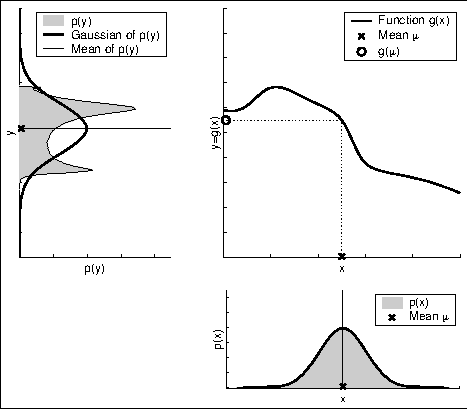
\includegraphics[width=0.5\columnwidth]{./images/nonlinear_transformation_of_a_gaussian.pdf}
	\end{figure}
\end{frame}

\begin{frame}
	\frametitle{Linearización en EKF}
	
	\begin{figure}[!h]
		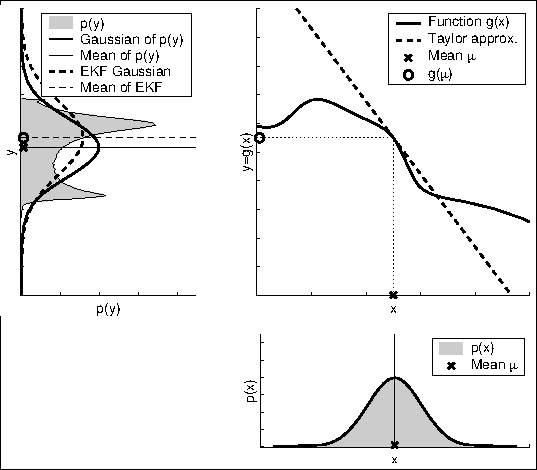
\includegraphics[width=0.5\columnwidth]{./images/linearization_applied_by_ekf.pdf}
	\end{figure}
\end{frame}


\begin{frame}
	\frametitle{Calidad de la Linearización en EKF}
	
	\begin{figure}[!h]
		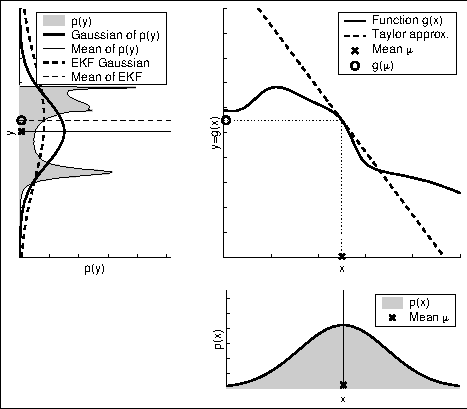
\includegraphics[width=0.5\columnwidth]{./images/dependency_approximation_quality_spread.pdf}
	\end{figure}
\end{frame}

\begin{frame}
	\frametitle{Calidad de la Linearización en EKF}
	
	\begin{figure}[!h]
		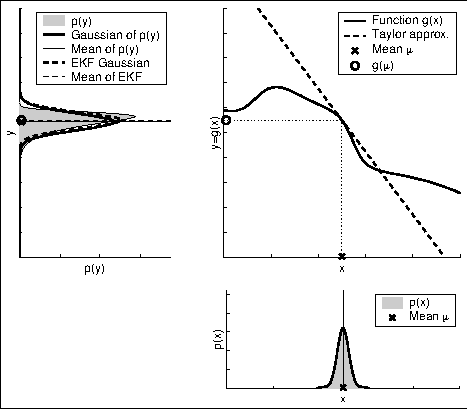
\includegraphics[width=0.5\columnwidth]{./images/dependency_approximation_quality_narrow.pdf}
	\end{figure}
\end{frame}


\begin{frame}
	\frametitle{Modelo de movimiento linearizado}
	\note{información extraida de https://youtu.be/PiCC-SxWlH8}
	
	\begin{itemize}
		\item Linearizar el modelo esta dado por:
	\begin{align*}
		p(\state_{t} | \controlCommand_{t}, \state_{t-1}) &\approx \det(2 \pi \motionParametersCovariance_{t})^{\frac{1}{2}}\\
		&\exp (-\dfrac{1}{2} (\state_{t} - \motionModelFunction{\controlCommand_{t}-\mu_{t-1}} - \motionModelJacobian_{t}(\state_{t-1}-\mu_{t-1}))^{\top}\\
		&\inverse{\motionParametersCovariance_{t}} (\state_{t} - \underbrace{\motionModelFunction{\controlCommand_{t},\mu_{t-1}} - \motionModelJacobian_{t} (\state_{t-1}-\mu_{t-1})}_{\text{modelo linearizado}}))
	\end{align*}
	
	\item $\motionParametersCovariance_{t}$ describe el ruido del movimiento
	\end{itemize}	
\end{frame}

\begin{frame}
	\frametitle{Modelo de observación linearizado}
	\note{información extraida de https://youtu.be/PiCC-SxWlH8}
	
	\begin{itemize}
		\item Linearizar el modelo esta dado por:
		\begin{align*}
			p(\observation_{t} | \state_{t}) &\approx \det(2 \pi \observationModelCovariance_{t})^{\frac{1}{2}}\\
			&\exp (-\dfrac{1}{2} (\observation_{t} - \observationModelFunction{\overline{\mu_{t}}} - \observationModelJacobian_{t}(\state_{t} - \overline{\mu_{t}}))^{\top}\\
			&\inverse{\observationModelCovariance_{t}} (\observation_{t} - \underbrace{\observationModelFunction{\overline{\mu_{t}}} - \observationModelJacobian_{t} (\state_{t}-\overline{\mu_{t}})}_{\text{modelo linearizado}}))
		\end{align*}
		
		\item $\observationModelCovariance_{t}$ describe el ruido de la medición
	\end{itemize}	
	
	
\end{frame}

\begin{frame}
	\frametitle{Algoritmo de Filtro de Kalman Extendido}
	\note{información extraída de https://youtu.be/PiCC-SxWlH8}
	
    \begin{algorithmic}[1]
    \Procedure{ExtendedKalmanFilter}{$\mu_{t-1}, \covariance_{t-1}, \controlCommand_{t}, \observation_{t}$}
        \State $\overline{\mu}_{t} = \motionModelFunction{\controlCommand_{t}, \mu_{t-1}}$
        \State $\overline{\covariance}_{t} = \motionModelJacobian_{t} \covariance_{t-1} \motionModelJacobian_{t}^{\top}+\motionParametersCovariance_{t}$
        \Statex
        \State $\kalmanGain_{t} = \overline{\covariance}_{t} \observationModelJacobian_{t}^{\top} (\observationModelJacobian_{t} \overline{\covariance}_{t}  \observationModelJacobian_{t} + \observationModelCovariance_{t})^{-1} $
        \State $\mu_{t} = \overline{\mu}_{t} + \kalmanGain_{t} (\observation_{t} - \observationModelFunction{\overline{\mu}_{t}})$
        \State $\covariance_{t} =  (I - \kalmanGain_{t} \observationModelJacobian_{t}) \overline{\covariance}_{t}$
        \State \Return $\mu_{t}, \covariance_{t}$
    \EndProcedure
    \end{algorithmic}
\end{frame}

\section{EKF Localización for feature-based map}

\begin{frame}
	\frametitle{Odometry as controls}
	\note{información extraida de https://youtu.be/PiCC-SxWlH8}
	
   	\begin{figure}[!h]
        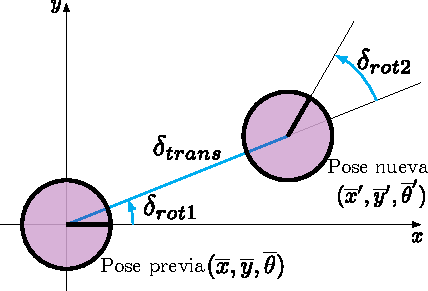
\includegraphics[width=0.6\columnwidth]{./images/odometry_as_controls.pdf}
    \end{figure}

    \begin{equation*}
        \controlCommand = (\delta_{rot1}, \delta_{trans}, \delta_{rot2})
    \end{equation*}
	
\end{frame}

\begin{frame}
	\frametitle{Motion model}
	\note{información extraida de https://youtu.be/PiCC-SxWlH8}
	
	\begin{itemize}
		\item Odometría de modelo de movimiento
		\begin{equation*}
			\begin{bmatrix}
				x^{\prime} \\
				y^{\prime} \\
				\theta^{\prime}
			\end{bmatrix} =
			\underbrace{
				\begin{bmatrix}
				x \\
				y \\
				\theta
			\end{bmatrix} +
			\begin{bmatrix}
				\delta_{trans}\cos(\theta+\delta_{rot_{1}}) \\
				\delta_{trans}\cos(\theta+\delta_{rot_{1}}) \\
				\delta_{rot_{1}} + \delta_{rot_{2}}
			\end{bmatrix}
			}_{\motionModelFunction{\controlCommand_{t}, \state_{t-1}}} + \normalDistribution{0}{\motionParametersCovariance_{t}}
		\end{equation*}
		\item Linearización
		\begin{equation*}
			\motionModelFunction{\controlCommand_{t}, \state_{t-1}} \approx 			\motionModelFunction{\controlCommand_{t}, \mu_{t-1}} + \motionModelJacobian_{t}(\state_{t-1}-\mu_{t-1})
		\end{equation*}
	\end{itemize}
	
\end{frame}

\begin{frame}
	\frametitle{Jacobianos del modelo de movimiento}
	\note{información extraida de https://youtu.be/PiCC-SxWlH8}
	Calculamos el Jacobiano con respecto al estado
	\begin{equation*}
		\motionModelJacobian_{t} = \dfrac{\delta\motionModelFunction{\controlCommand_{t},\mu_{t-1}}}{\delta \state_{t-1}} =
		\begin{bmatrix}
			\dfrac{\delta x^{\prime}}{\delta \mu_{t-1,x}} & \dfrac{\delta x^{\prime}}{\delta \mu_{t-1,y}} & \dfrac{\delta x^{\prime}}{\delta \mu_{t-1,\theta}}\\
			\dfrac{\delta y^{\prime}}{\delta \mu_{t-1,x}} & \dfrac{\delta y^{\prime}}{\delta \mu_{t-1,y}} & \dfrac{\delta y^{\prime}}{\delta \mu_{t-1,\theta}}\\
			\dfrac{\delta \theta^{\prime}}{\delta \mu_{t-1,x}} & \dfrac{\delta \theta^{\prime}}{\delta \mu_{t-1,y}} & \dfrac{\delta \theta^{\prime}}{\delta \mu_{t-1,\theta}}\\
		\end{bmatrix}
	\end{equation*}

	\begin{equation*}
	\motionModelJacobian_{t} = 
	\begin{bmatrix}
		1 & 0 & -\delta_{trans} \sin(\theta + \delta_{rot_{1}})\\
		0 & 1 & \delta_{trans} \cos(\theta + \delta_{rot_{1}})\\
		0 & 0 & 1\\
	\end{bmatrix}
	\end{equation*}
\end{frame}

\begin{frame}
	\frametitle{Jacobianos del modelo de movimiento}
	\note{información extraida de https://youtu.be/PiCC-SxWlH8}
	Calculamos el Jacobiano con respecto al comando de control
	\begin{equation*}
		\motionModelJacobianControl{t} = \dfrac{\delta\motionModelFunction{\controlCommand_{t},\mu_{t-1}}}{\delta \controlCommand_{t}} =
		\begin{bmatrix}
			\dfrac{\delta x^{\prime}}{\delta \controlCommand_{t,\delta_{rot_{1}}}} & \dfrac{\delta x^{\prime}}{\delta \controlCommand_{t,\delta_{trans}}} & \dfrac{\delta x^{\prime}}{\delta \controlCommand_{t,\delta_{rot_{2}}}}\\
			\dfrac{\delta y^{\prime}}{\delta \controlCommand_{t,\delta_{rot_{1}}}} & \dfrac{\delta y^{\prime}}{\delta \controlCommand_{t,\delta_{trans}}} & \dfrac{\delta y^{\prime}}{\delta \controlCommand_{t,\delta_{rot_{2}}}}\\
			\dfrac{\delta \theta^{\prime}}{\delta \controlCommand_{t,\delta_{rot_{1}}}} & \dfrac{\delta \theta^{\prime}}{\delta \controlCommand_{t,\delta_{trans}}} & \dfrac{\delta \theta^{\prime}}{\delta \controlCommand_{t,\delta_{rot_{2}}}}
		\end{bmatrix}
	\end{equation*}
	
	\begin{equation*}
		\motionModelJacobianControl_{t} = 
		\begin{bmatrix}
			-\delta_{trans} \sin(\theta + \delta_{rot_{1}}) & \cos(\theta + \delta_{rot_{1}}) & 0\\
			\delta_{trans} \cos(\theta + \delta_{rot_{1}}) & \sin(\theta + \delta_{rot_{1}}) & 0\\
			0 & 0 & 1\\
		\end{bmatrix}
	\end{equation*}
\end{frame}

\begin{frame}
	\frametitle{Modelo de observación}
	\note{información extraida de https://youtu.be/PiCC-SxWlH8}
	\begin{itemize}
	\item Modelo de distancia y orientación (range-bearing model)
	\begin{equation*}
		\observation_{t}^{i} =
		\begin{bmatrix}
			r_{t}^{i}\\
			\phi_{t}^{i} 
		\end{bmatrix} =
		\begin{bmatrix}
			\sqrt{(m_{j,x}-x)^{2} + (m_{j,y}-y)^{2}}\\
			\atantwo(m_{j,y}-y, m_{j,x}-x) -\theta
		\end{bmatrix}
		+ \normalDistribution{0}{\observationModelCovariance_{t}}		
	\end{equation*}
	
	\item Linearización
	\begin{equation*}
	\observationModelFunction{\state_{t}, m} \approx 			\observationModelFunction{\overline{\mu}_{t}} + \observationModelJacobian_{t}^{i}(\state_{t}-\overline{\mu}_{t})
	\end{equation*}
	\end{itemize}
	
\end{frame}

\begin{frame}
	\frametitle{Jacobianos del modelo de observación}
	\note{información extraida de https://youtu.be/PiCC-SxWlH8}
	Calculamos el Jacobiano con respecto al estado
	\begin{equation*}
		\observationModelJacobian_{t} = \dfrac{\delta\observationModelFunction{\overline{\mu}_{t},m}}{\delta \state_{t-1}} =
		\begin{bmatrix}
			\dfrac{\delta r_{t}^{i}}{\delta \overline{\mu}_{t,x}} & \dfrac{\delta r_{t}^{i}}{\delta \overline{\mu}_{t,y}} & \dfrac{\delta r_{t}^{i}}{\delta \overline{\mu}_{t,\theta}}\\
			\dfrac{\delta \phi_{t}^{i}}{\delta \overline{\mu}_{t,x}} & \dfrac{\delta \phi_{t}^{i}}{\delta \overline{\mu}_{t,y}} & \dfrac{\delta \phi_{t}^{i}}{\delta \overline{\mu}_{t,\theta}}
		\end{bmatrix}
	\end{equation*}
	
	\begin{equation*}
		\observationModelJacobian_{t}^{i} = 
		\begin{bmatrix}
			-\dfrac{m_{j,x} - \overline{\mu}_{t,x}}{\sqrt{q}} & -\dfrac{m_{j,y} - \overline{\mu}_{t,y}}{\sqrt{q}}  & 0\\
			-\dfrac{m_{j,y} - \overline{\mu}_{t,y}}{q}  & -\dfrac{m_{j,x} - \overline{\mu}_{t,x}}{q}  & -1
		\end{bmatrix}
	\end{equation*}
	donde
	\begin{equation*}
		q = (m_{j,x}-\overline{\mu}_{t,x})^{2} + (m_{j,y}-\overline{\mu}_{t,y})^{2}
	\end{equation*}
\end{frame}

\begin{frame}
	\frametitle{Algoritmo de Filtro de Kalman Extendido}
	\note{información extraida de https://youtu.be/PiCC-SxWlH8}
	
 	\begin{algorithmic}[1]
		\State ExtendedKalmanFilter({$\mu_{t-1}, \covariance_{t-1}, \controlCommand_{t}, \observation_{t}$, $c_{t}$, $m$})
		\State $\theta = \mu_{t-1,\theta}$
		
		\State $
			\motionModelJacobian_{t} = 
			\begin{bmatrix}
				1 & 0 & -\delta_{trans} \sin(\theta + \delta_{rot_{1}})\\
				0 & 1 & \delta_{trans} \cos(\theta + \delta_{rot_{1}})\\
				0 & 0 & 1\\
			\end{bmatrix}
			   $
		\State $
			\motionModelJacobianControl_{t} = 
			\begin{bmatrix}
				-\delta_{trans} \sin(\theta + \delta_{rot_{1}}) & \cos(\theta + \delta_{rot_{1}}) & 0\\
				\delta_{trans} \cos(\theta + \delta_{rot_{1}}) & \sin(\theta + \delta_{rot_{1}}) & 0\\
				0 & 0 & 1\\
			\end{bmatrix}
         	   $
		\State $
			\motionModelCovariance_{t} = 
			\begin{bmatrix}
				\alpha_{1}\delta^{2}_{rot_{1}} + \alpha_{2}\delta^{2}_{trans} & 0 & 0\\
				0 & \alpha_{3} \delta^{2}_{trans} + \alpha_{4} \left( \delta^{2}_{rot_{1}} + \delta^{2}_{rot_{2}} \right) & 0\\
				0 & 0 & \alpha_{1}\delta^{2}_{rot_{1}} + \alpha_{2}\delta^{2}_{trans}\\
			\end{bmatrix}
			  $
		\State $\overline{\mu}_{t} = \mu_{t-1} + 
			\begin{bmatrix}
			\delta_{trans}\cos(\theta+\delta_{rot_{1}}) \\
			\delta_{trans}\cos(\theta+\delta_{rot_{1}}) \\
			\delta_{rot_{1}} + \delta_{rot_{2}}
		\end{bmatrix}$
		\State $\overline{\covariance}_{t} = \motionModelJacobian_{t} \covariance_{t-1} \motionModelJacobian_{t}^{\top}+\motionModelJacobianControl_{t} \motionModelCovariance_{t} \motionModelJacobianControl_{t}^{\top}$
	\end{algorithmic}
	
\end{frame}

\begin{frame}
	\frametitle{Prediction step}
	\note{información extraida de https://youtu.be/PiCC-SxWlH8}
	
	\begin{figure}[!h]
		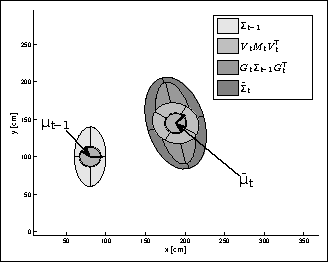
\includegraphics[width=0.5\columnwidth]{./images/prediction_step.pdf}
	\end{figure}
	
\end{frame}

\begin{frame}
	\frametitle{Algoritmo de Filtro de Kalman Extendido}
	\note{información extraida de https://youtu.be/PiCC-SxWlH8}
	\footnotesize
 	\begin{algorithmic}[1]
		\State
		$ \observationModelCovariance_{t} =
			\begin{bmatrix}
				\sigma_{r}^{2} & 0\\
				0 & \sigma_{\phi}^{2}
			\end{bmatrix}
		$
		\For todos los features observados $z_{t}^{i} = (r_{t}^{i}, \phi_{t}^{i})^{\top}$
		
		\State $ j = c_{t}^{i}$
		\State $ q = (m_{j,x}-\overline{\mu}_{t,x})^{2} + (m_{j,y}-\overline{\mu}_{t,y})^{2} $
		\State
		$ \hat{\observation}_{t}^{i} =
			\begin{bmatrix}
				\sqrt{q}\\
				\atantwo(m_{j,y}-\overline{\mu}_{t,y}, m_{j,x}-\overline{\mu}_{t,x}) - \overline{\mu}_{t,\theta}
			\end{bmatrix}
		$
		\State
		$ \observationModelJacobian_{t}^{i} = 
			\begin{bmatrix}
				-\dfrac{m_{j,x} - \overline{\mu}_{t,x}}{\sqrt{q}} & -\dfrac{m_{j,y} - \overline{\mu}_{t,y}}{\sqrt{q}}  & 0\\
				-\dfrac{m_{j,y} - \overline{\mu}_{t,y}}{q}  & -\dfrac{m_{j,x} - \overline{\mu}_{t,x}}{q}  & -1
			\end{bmatrix}
		$
		
		\State $S_{t}^{i} = \observationModelJacobian_{t}^{i} \overline{\covariance}_{t} \observationModelJacobian_{t}^{i^{\top}} + \observationModelCovariance_{t} $

		\State $\kalmanGain_{t}^{i} = \overline{\covariance}_{t} {\observationModelJacobian_{t}^{i}} \overline{\covariance}_{t} \observationModelJacobian_{t}^{i^{\top}} S_{t}^{i^{-1}} $
		\State $\overline{\mu}_{t} = \overline{\mu}_{t} + \kalmanGain_{t}^{i}(\observation_{t} - \hat{\observation}_{t}^{i})$
		\State $\overline{\covariance}_{t} = (I - \kalmanGain_{t}^{i}\observationModelJacobian_{t}^{i})\overline{\covariance}_{t}$
		
		\EndFor
		\State $\mu_{t} = \overline{\mu}_{t}$
		\State $\covariance_{t} = \overline{\covariance}_{t}$
		
		\State \Return $\mu_{t}, \covariance_{t}$
	\end{algorithmic}
	
	
\end{frame}

\begin{frame}
	\frametitle{Medición esperada}
	\note{información extraida de https://youtu.be/PiCC-SxWlH8}
	
	\begin{figure}[!h]
		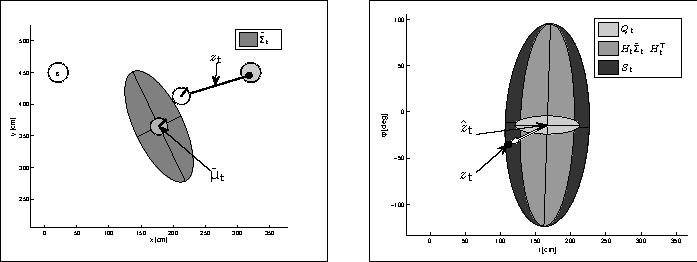
\includegraphics[width=\columnwidth]{./images/measurement_prediction.pdf}
	\end{figure}
	
\end{frame}

\begin{frame}
	\frametitle{Correction step}
	\note{información extraida de https://youtu.be/PiCC-SxWlH8}
	
	\begin{figure}[!h]
			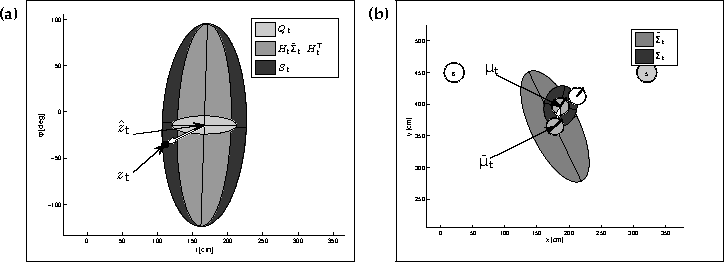
\includegraphics[width=\columnwidth]{./images/correction_step.pdf}
	\end{figure}
	
\end{frame}

\begin{frame}
	\frametitle{Ejemplo: EKF Localization 2D}
	\note{información extraida de libro Probabilistic Robotics}
	
	\begin{figure}[!h]
		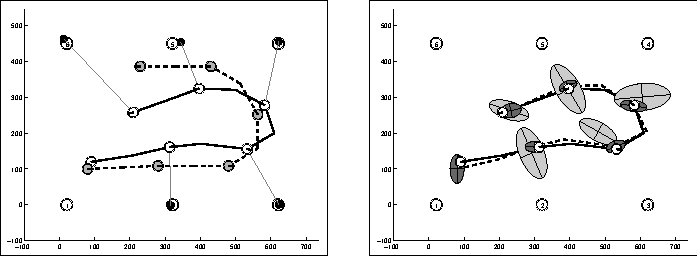
\includegraphics[width=\columnwidth]{./images/ekf_localization_example.pdf}
	\end{figure}
	
\end{frame}

\begin{frame}
	\frametitle{Resumen de EKF}
	\note{información extraida de https://youtu.be/PiCC-SxWlH8}
	
	\begin{itemize}
		\item Es una extensión del Filtro de Kalman
		\item Una forma de trabajar con no-lineridades
		\item Realiza linearizaciones locales
		\item Funciona bien en la práctica para casos moderadamente no lineales
		\item Grandes incertidumbres conllevan un incremento del error
	\end{itemize}
	
\end{frame}

